\documentclass[12pt,fleqn]{article}\usepackage{../../common}
\begin{document}
Genel Makroekonomi

Paranin Miktar Teorisi (Quantity Theory of Money) 

Bir liran�n g�nl�k hayat i�inde dola��m�n� d���nelim. Ben gidiyorum mesela
k��e ba��ndaki sat�c�dan bir po�a�a al�yorum. Bu sat�c� liray� k�z�na
veriyor, k�z�da onu lunaparkta ata binmek i�in kullan�yor. At� kiralayan
Ali liray� eve g�t�r�yor, bir s�re koltuk alt�nda kaybediyor, tekrar
buluyor, sonra seyahat edip yabanc� bir �lkede onu kahve almak i�in
kullan�yor. Butun bir sene icinde bu lira uc kere harcanmis oluyor. 

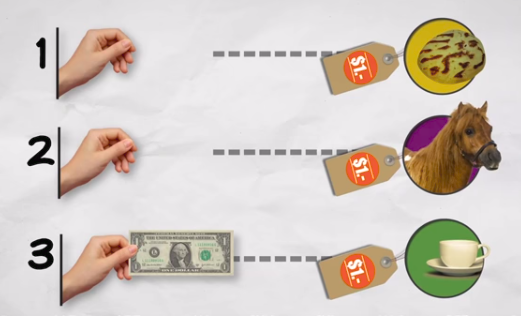
\includegraphics[width=20em]{tser_macro_01.png}



































\newpage

$$ \Delta p_R + \Delta y = \Delta c_R$$

$$ \Delta (P_RY) = V_R\Delta C_R$$

$$ \Delta (P_RY) = \Delta c + \Delta i + \Delta g + \Delta nx $$

$$ \Delta c + \Delta i + \Delta g + \Delta nx = V_R\Delta C_R$$

$$ \Delta (c +  i +  nx) = V_R\Delta C_R - \Delta g$$

$$ \Delta GDP_t = \Delta C_{Rt-1}$$

$$ \Delta GDP_t + \Delta GDP_{t-1} = \Delta C_{Rt-1} + \Delta GDP_{t-1} $$

$$ \Delta GDP_t + \Delta GDP_{t-1} = \Delta C_{Rt-1} + \Delta C_{Rt-2}  $$

$$ \Delta GDP_t = - \Delta GDP_{t-1} + \Delta C_{Rt-1} + \Delta C_{Rt-2}  $$


$c$ nominal consumption 

$i$ nominal government expenditure

$i$ nominal investment 

$nx$ nominal net exports

$$ \Delta GDP_t = 
\alpha + \beta_1 \Delta GDP_{t-1} + 
\gamma_0 \Delta C_{Rt} + \gamma_3 \Delta C_{Rt-3} + \epsilon_t 
$$

$$ 
\Delta (c_t + i_t + nx_t) = 
\alpha + \beta_0 \Delta g_t + \beta_1 \Delta GDP_{t-1} + 
\gamma_0 \Delta C_{Rt} + \gamma_3 \Delta C_{Rt-3} + \epsilon_t 
$$

$$ 
\Delta (c_t + i_t + nx_t) =  
\alpha + \beta_0 \Delta g_t + 
\beta_1 \Delta GDP_{t-1} +  
\gamma_0 \Delta C_{Rt} + 
 \gamma_0 \Delta C_{Rt-1} + ...  + \epsilon_t 
$$


\begin{minted}[fontsize=\footnotesize]{python}
import pandas as pd
df = pd.read_csv('data.csv',parse_dates=True)
df = df.dropna(axis=0)
df = df.set_index('DATE')
df['govexp'] = (df['gov1exp'] + df['gov2exp']) 
df['lhs'] = (df.consump + df.invest + df.netexp).pct_change()
df['dgt'] = df.govexp.pct_change()
df['dcrt'] = (df.nonfinloan - df.constructloan).pct_change()
df['dcrt1'] = df.dcrt.shift(1)
df['dcrt2'] = df.dcrt.shift(2)
df['dcrt3'] = df.dcrt.shift(3)
df['dcrt4'] = df.dcrt.shift(4)
df['dgdpt'] = df.gdp.pct_change()
df['dgdpt1'] = -1 * df.dgdpt.shift(1)
df['dgdpt2'] = -1 * df.dgdpt.shift(2)
df['dgdpt3'] = -1 * df.dgdpt.shift(3)
df = df.dropna(axis=0)
print (df.tail(5))
\end{minted}

\begin{verbatim}
            consump   gov1exp   gov2exp    invest   netexp        gdp  \
DATE                                                                    
2016-01-01  109.981  4176.842  2650.478  2849.839 -526.236  18325.187   
2016-04-01  110.550  4164.494  2673.472  2830.237 -501.567  18538.039   
2016-07-01  111.029  4232.902  2691.437  2847.246 -492.834  18729.130   
2016-10-01  111.577  4266.220  2712.709  2905.720 -564.320  18905.545   
2017-01-01  112.192  4320.538  2737.536  2896.996 -582.844  19057.705   

            nonfinloan  constructloan    govexp       lhs       dgt      dcrt  \
DATE                                                                            
2016-01-01   27236.607      3889.7280  6827.320 -0.014302  0.010270  0.008822   
2016-04-01   27550.841      3959.9659  6837.966  0.002316  0.001559  0.010451   
2016-07-01   27895.222      4031.5850  6924.339  0.010750  0.012631  0.011562   
2016-10-01   28108.440      4098.3063  6978.929 -0.005055  0.007884  0.006139   
2017-01-01   28421.574      4132.2395  7058.074 -0.010857  0.011341  0.011628   

               dcrt1     dcrt2     dcrt3     dcrt4     dgdpt    dgdpt1  \
DATE                                                                     
2016-01-01  0.007478  0.008217  0.014951  0.008115  0.002076 -0.003266   
2016-04-01  0.008822  0.007478  0.008217  0.014951  0.011615 -0.002076   
2016-07-01  0.010451  0.008822  0.007478  0.008217  0.010308 -0.011615   
2016-10-01  0.011562  0.010451  0.008822  0.007478  0.009419 -0.010308   
2017-01-01  0.006139  0.011562  0.010451  0.008822  0.008048 -0.009419   

              dgdpt2    dgdpt3  
DATE                            
2016-01-01 -0.007432 -0.012224  
2016-04-01 -0.003266 -0.007432  
2016-07-01 -0.002076 -0.003266  
2016-10-01 -0.011615 -0.002076  
2017-01-01 -0.010308 -0.011615  
\end{verbatim}

\begin{minted}[fontsize=\footnotesize]{python}
import statsmodels.formula.api as smf
results = smf.ols('lhs ~ dgt +  dgdpt1 + dcrt  + dcrt2 ', data=df).fit()
print results.summary()
\end{minted}

\begin{verbatim}
                            OLS Regression Results                            
==============================================================================
Dep. Variable:                    lhs   R-squared:                       0.102
Model:                            OLS   Adj. R-squared:                  0.086
Method:                 Least Squares   F-statistic:                     6.297
Date:                Sun, 13 May 2018   Prob (F-statistic):           8.14e-05
Time:                        16:46:50   Log-Likelihood:                 437.96
No. Observations:                 226   AIC:                            -865.9
Df Residuals:                     221   BIC:                            -848.8
Df Model:                           4                                         
Covariance Type:            nonrobust                                         
==============================================================================
                 coef    std err          t      P>|t|      [95.0% Conf. Int.]
------------------------------------------------------------------------------
Intercept      0.0100      0.006      1.810      0.072        -0.001     0.021
dgt           -0.3688      0.173     -2.133      0.034        -0.710    -0.028
dgdpt1        -0.6514      0.293     -2.222      0.027        -1.229    -0.074
dcrt           0.8709      0.344      2.533      0.012         0.193     1.548
dcrt2         -1.1395      0.327     -3.485      0.001        -1.784    -0.495
==============================================================================
Omnibus:                        2.420   Durbin-Watson:                   2.230
Prob(Omnibus):                  0.298   Jarque-Bera (JB):                2.437
Skew:                          -0.002   Prob(JB):                        0.296
Kurtosis:                       3.509   Cond. No.                         188.
==============================================================================

Warnings:
[1] Standard Errors assume that the covariance matrix of the errors is correctly specified.
\end{verbatim}

















[1] {\em Quantity Theory of Money}, \url{https://youtu.be/q59tZKP0HME}

\end{document}

























